\documentclass[10pt]{article}
\usepackage{url}
\usepackage{amsmath}
\usepackage{graphicx}
\usepackage{float}
\usepackage[font=footnotesize]{caption}
\usepackage{vmargin}
\usepackage{multirow}
\usepackage{ctable}
\usepackage{xcolor}
\usepackage{listings}
\usepackage{hyperref}
\usepackage{listings}
\usepackage{tabularx}

%Unidades SI
\usepackage{siunitx}
\usepackage{mathtools}
\usepackage{setspace}
\usepackage{fontspec}
\usepackage{xcolor}
\usepackage{titlesec}
\usepackage{parskip}
\usepackage{subfig}
\usepackage{fancyhdr}
\usepackage{inputenc}
\usepackage{lipsum}

% more packages
\usepackage{subfig}
\usepackage[super]{nth}
\usepackage{array}
\usepackage{multirow}
\usepackage{arydshln}
\usepackage{makecell}

% \usepackage{biblatex}
\newcommand{\vertfig}[2][]{%
  \begin{minipage}{5in}\subfloat[#1]{#2}\end{minipage}}
\newcommand{\horizfig}[2][]{%
  \begin{minipage}{3in}\subfloat[#1]{#2}\end{minipage}}
%New colors defined below
\definecolor{codegreen}{rgb}{0,0.6,0}
\definecolor{codegray}{rgb}{0.5,0.5,0.5}
\definecolor{codepurple}{rgb}{0.58,0,0.82}
\definecolor{backcolour}{rgb}{0.95,0.95,0.92}

\lstdefinestyle{mystyle}{
    backgroundcolor=\color{backcolour},
    commentstyle=\color{codegreen},
    keywordstyle=\color{magenta},
    numberstyle=\tiny\color{codegray},
    stringstyle=\color{codepurple},
    basicstyle=\ttfamily\footnotesize,
    breakatwhitespace=false,
    breaklines=true,
    captionpos=b,
    keepspaces=true,
    numbers=left,
    numbersep=5pt,
    showspaces=false,
    showstringspaces=false,
    showtabs=false,
    tabsize=2
    }

\lstset{style=mystyle}
\lstnewenvironment{code}{\lstset{language=C, basicstyle=\ttfamily, frame=single, numbers=left}}{}
\setlength{\parindent}{0pt}
\graphicspath{ {./imagens/} }
% \addbibresource{references.bib}

\newcommand{\polish}[1]{\textcolor{red}{#1}}

%Capa%
\title{
\centering

\includegraphics[width=0.35\textwidth]{capa/logo.png}\par\vspace{1cm}
\normalfont \large 
Instituto Superior Técnico\\
\vspace{5mm}
\normalsize 2023/2024 - \nth{4} Period \\
\vspace{15mm}
\huge \textbf{Computational Intelligence for the Internet of Things}\\
\vspace{15mm}
\huge {\nth{1} project}\\
\huge {Fuzzy Systems and Neural Networks}\\
\LARGE {Part I}\\
\LARGE {Fuzzy System}\\
\normalsize
\vspace{5mm}
\textbf{Prof:} Joao Paulo Carvalho\\
\vspace{15mm}
Group 3
\vspace{5mm}
\begin{enumerate}
    \centering
    \item \textbf{No:} 94230  \hspace{2cm} \textbf{Name:} Samuel Barata
    \item \textbf{No:} 96765  \hspace{2cm} \textbf{Name:} Sandra Castilho
\end{enumerate}
\vspace{25mm}
}

\begin{document}

\maketitle

% The report should contain the following:
% Indicate the “architecture” of your FIS and the rationale you used to build it.
% Include all the membership functions, linguistic terms, and rules.
% Illustrative graphics are encouraged.
% Also describe how you tested the system to see if it performed as you envisioned it, and any tunning and modifications you made until you reached the final version.
% Add the results you obtained.

\section{Introduction}
\normalfont
The explosive growth of Internet of Things (IoT) devices has resulted in a high volume of data being generated, but most of it is not exploited or used at all, since sending all that device-generated data to a centralized data center or to the cloud causes bandwidth and latency issues.

One solution to this problem is to take advantage of the edge devices, using their spare computing capabilities to enable faster and more comprehensive data analysis, without exchange the data over to the cloud (which also reduces the network load).

However, one should be aware not to exhaust the edge resources, to not compromise the normal operation of the edge devices or the network bandwidth.

The objective of this project is to build an intelligent system that manages the computing load assigned for Edge computing tasks on an Edge device (CLP), without compromising the main role of the device. This consists on using edge devices to compute as much as it possibly can without affecting its own edge functionality and without increasing congestion on the network.

\section{Fuzzy System}
\label{sec:fuzzy_system}
\subsection{Introduction}

The objective is to create a Fuzzy Inference System (FIS) capable of controlling the variation of the Computing Load Percentage (CLPVariation), given some system parameters as input (such as memory, processor, network, etc...).
It is assumed that when the device is operating as a pure Edge device (i.e., CLP
= 0), only networking duties (including routing data to the cloud) are performed.

\subsection{Architecture and Decisions}
% Include all the membership functions, linguistic terms, and rules. Illustrative graphics are encouraged

To help construct the fuzzy system, we have the following system features:
\begin{itemize}
    \item Memory Usage
    \item Processor Load
    \item Input network throughput
    \item Output network throughput
    \item Available output bandwidth
    \item Latency
\end{itemize}
Each feature is a one-minute average, and for each one, the variation rate is also available.

\subsection{Variables}

Because Fuzzy systems' rule base size increases exponentially with the number of inputs, we began by selecting the important features of the system to use, and also how to combine/group them in smaller fuzzy systems.

We decided not to use the Variation values, as it would overcomplicate the system, and the insights that we would get from them would not be very useful. For example, it was hypothesized to group the Processor Load and its Variation, considering that a positive variation for a "long" period of time would mean a high load on the device and the CLP should decrease. However, we do not have a way to record the state, and knowing the current state of the processor load of the device is enough, as we want to keep its usage around a certain value (70\%-80\%).

Because the \textit{Memory Usage} and \textit{Processor Load} are a good indicative of the current performance of the system, and since either of them having extremely high usage will have a great impact on the device performance, we joined these two features to be the inputs of a fuzzy system (FS\_HDR) that have as output \textit{Hardware Resources}.

On the same train of thought, we tried to combine the network features (\textit{Output Throughput, Available Output Bandwidth, Input Throughput} and \textit{Latency}) on a fuzzy system whose output was \textit{Network Usage}, to have an idea of how congested the network could be.

Finally, we computed the value for the CLP based on the \textit{Hardware Resources} and \textit{Network Usage}.

The original architecture is presented in figure \ref{fig:originalFS}.

\begin{figure}[!htb]
    \centering
    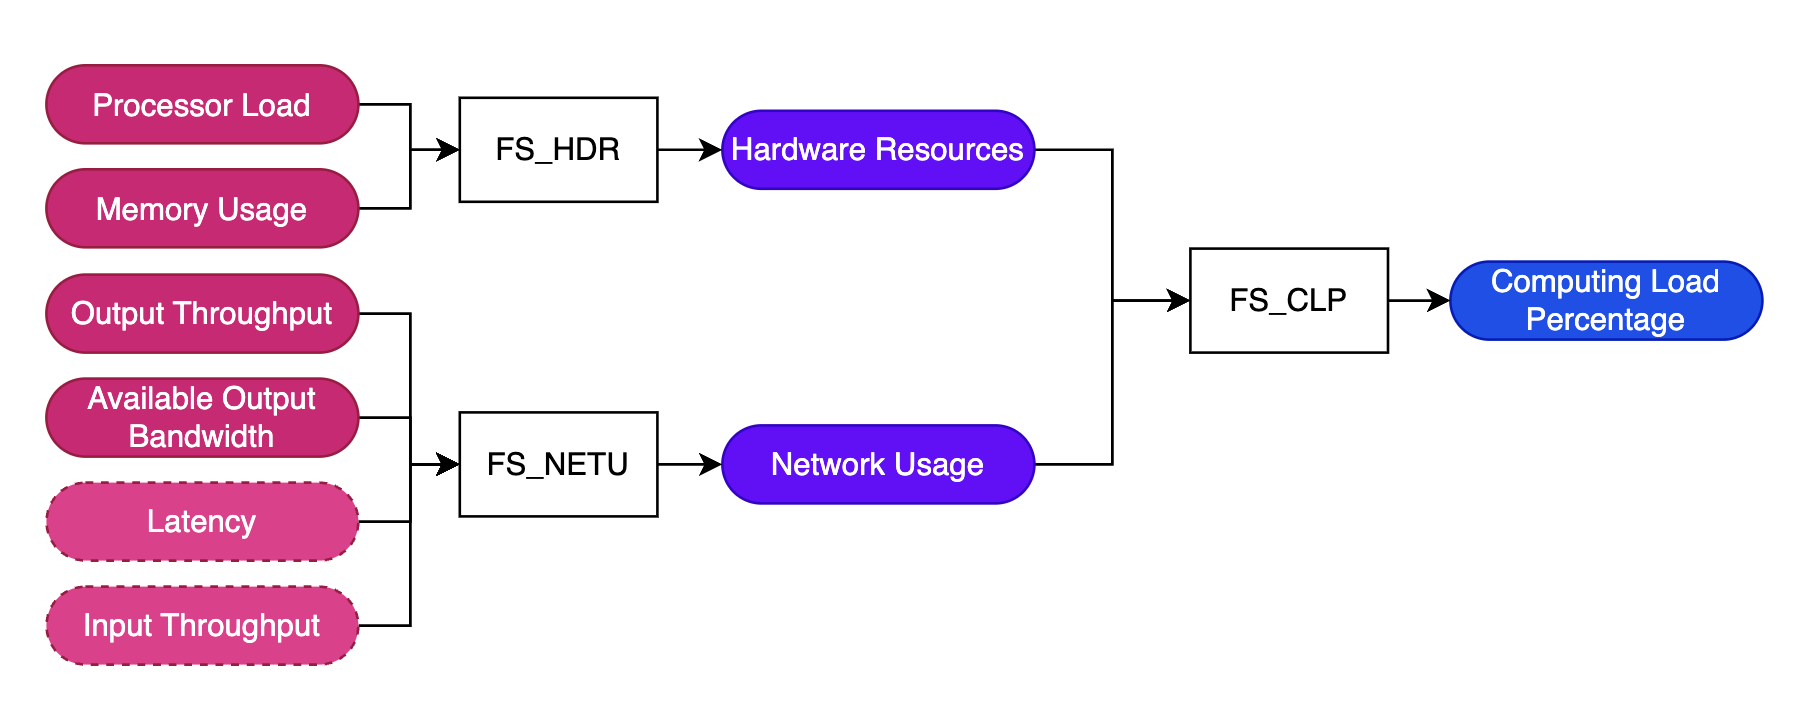
\includegraphics[width=\textwidth, height=\textheight, keepaspectratio]{images/fuzzy_systems_og.png}
    \caption{Original Fuzzy systems architecture}
    \label{fig:originalFS}
\end{figure}

We experimented with combining the features of the \textit{Network Usage} and reached the following conclusions:
\begin{itemize}
    \item Because the input network and the output network are not necessarily correlated, we shouldn't join them in an "outer" fuzzy system, but instead consider the \textit{Input Throughput} in the final Fuzzy System (the one that computes the CLP), as a "tiebreaker" of Hardware and Network load, as high \textit{Input Throughput} implies more data to be processed - and thus an incentive to process it locally. However, while constructing the FAM (Fuzzy Associative Memory) for it, we concluded that its weight was meaningless, and discarded it.
    \item \textit{Latency} was discarded from the \textit{Network Usage}, considering that the packets should reach their destination anyway with high latency, but a congested link will mean loss of packets, and that is worse than a slow link. However, the values that we were getting for the CLP value when considering the \textit{Latency} as an input of the final fuzzy system were not satisfactory, and decided to discard it as well.
\end{itemize}

In the end, we ended up with a fuzzy system that computes the \textit{Output Congestion} (FS\_OUTC), using as input the \textit{Output Throughput} and \textit{Available Output Bandwidth}.
The value for the CLP is then based on the \textit{Hardware Resources} and \textit{Output Congestion}.

The final architecture of the project is presented in figure \ref{fig:finalFS}.

\begin{figure}[!htb]
    \centering
    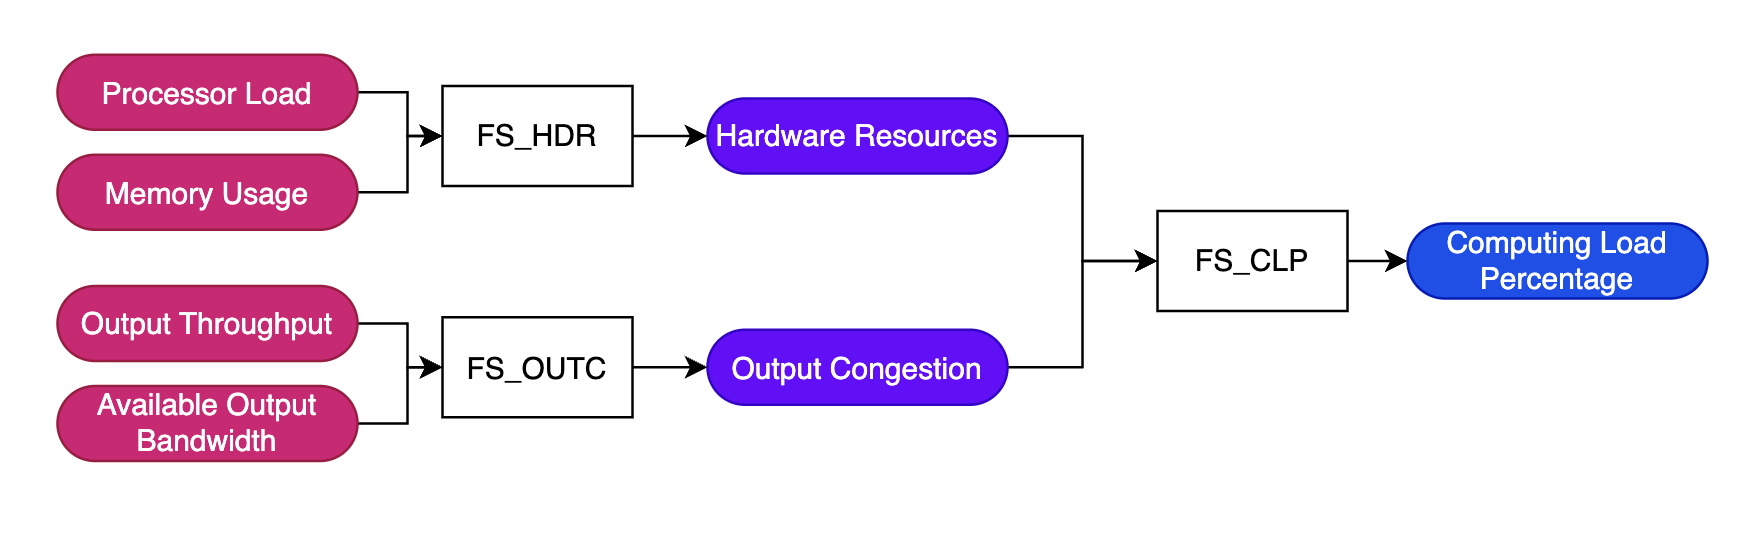
\includegraphics[width=\textwidth, height=\textheight, keepaspectratio]{images/fuzzy_systems_final.png}
    \caption{Final Fuzzy systems architecture}
    \label{fig:finalFS}
\end{figure}


\subsubsection{Linguistic Terms \& Membership Functions (Fuzzy Sets)}
We chose the Linguistic Terms "High", "Medium" and "Low" for all the input Fuzzy Sets, and "Increase", "Maintain" and "Decreased" for the output \textit{CLP Variation}, and to allow a better categorization of the fuzzy sets, we decided to use trapezoids over triangles.
After testing the fuzzy systems, it was necessary to add more members to some fuzzy systems, as shown in the membership functions below (for example, adding a "very high" member to the \textit{Processor Load}, or adding "decrease much" and "increase much" members to the \textit{CLP Variation}).

The Membership Functions for our fuzzy systems are presented in the figures \ref{fig:FS_HDR_FSETS}, \ref{fig:FS_OUTC_FSETS} and \ref{fig:FS_CLP_FSETS}.

\begin{figure}[!htb]
    \centering
    \hspace*{-1cm}

    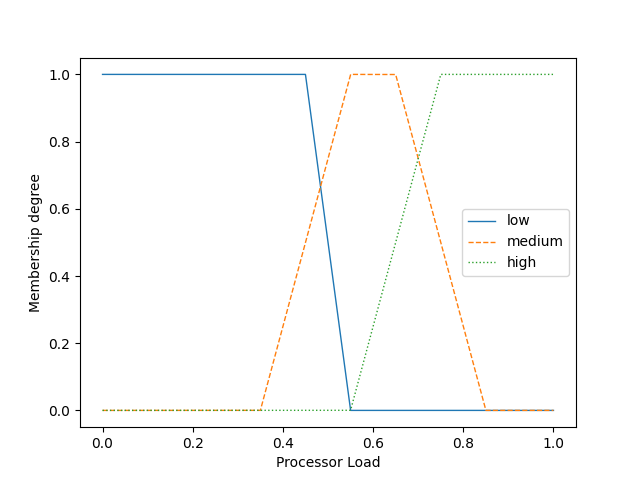
\includegraphics[width=.33\textwidth]{images/plots/ProcessorLoad.png}\hfill
    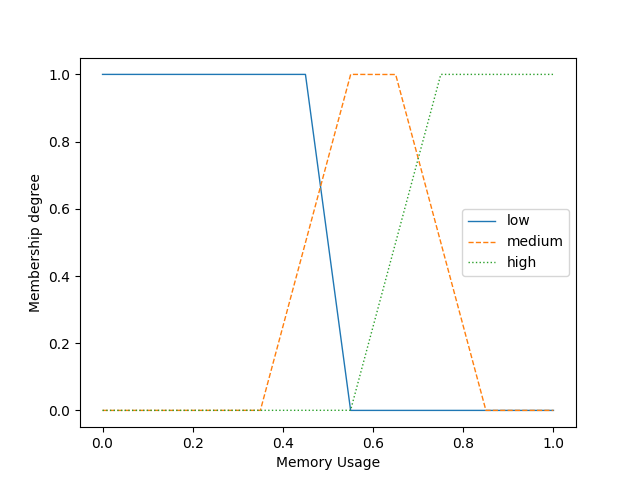
\includegraphics[width=.33\textwidth]{images/plots/MemoryUsage.png}\hfill
    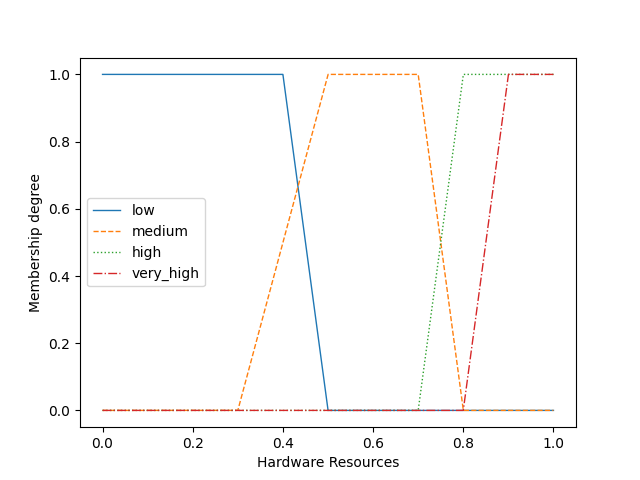
\includegraphics[width=.33\textwidth]{images/plots/CpuMemCLP.png}

    \hspace*{-1cm}
    \caption{Membership functions for the "Hardware Resources" Fuzzy System}
    \label{fig:FS_HDR_FSETS}
\end{figure}

\begin{figure}[!htb]
    \centering
    \hspace*{-1cm}

    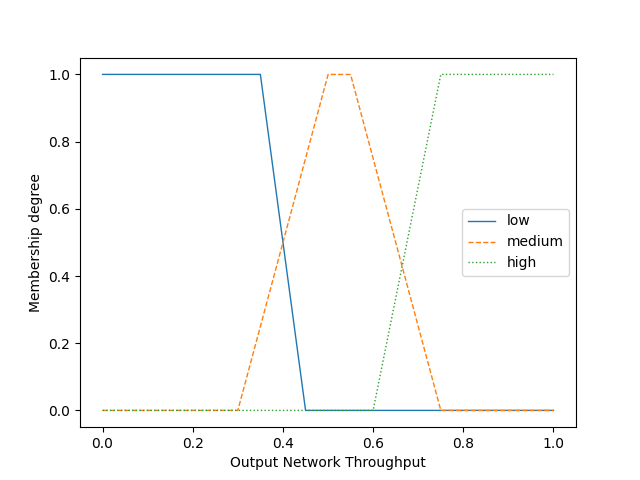
\includegraphics[width=.33\textwidth]{images/plots/OutNetThroughput.png}\hfill
    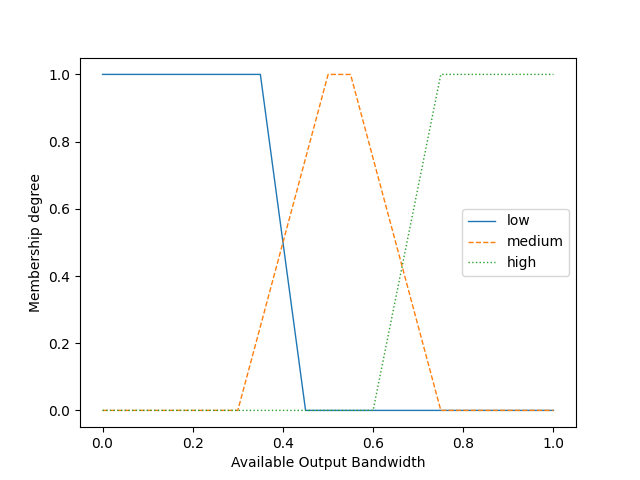
\includegraphics[width=.33\textwidth]{images/plots/AvailOutBandwidth.png}\hfill
    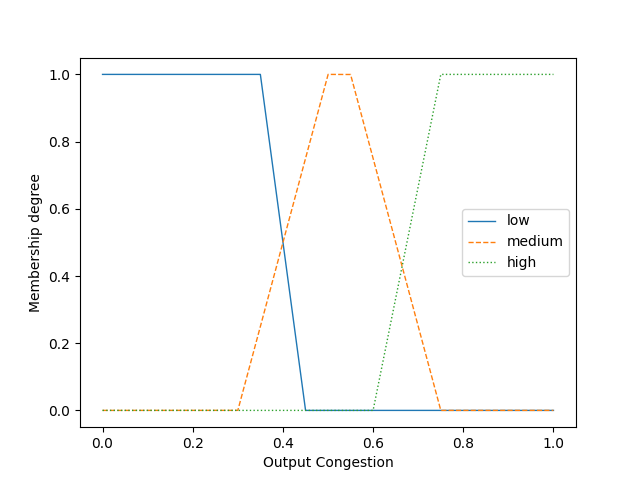
\includegraphics[width=.33\textwidth]{images/plots/OutCongestion.png}

    \hspace*{-1cm}
    \caption{Membership functions for the "Output Congestion" Fuzzy System}
    \label{fig:FS_OUTC_FSETS}
\end{figure}

\begin{figure}[!htb]
    \centering
    \hspace*{-1cm}

    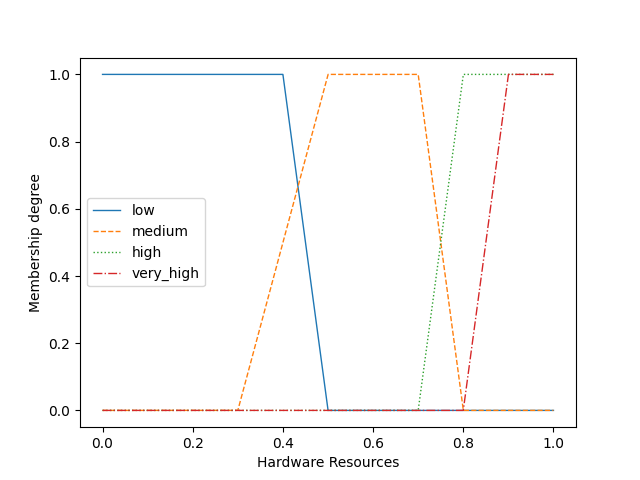
\includegraphics[width=.33\textwidth]{images/plots/CpuMem.png}\hfill
    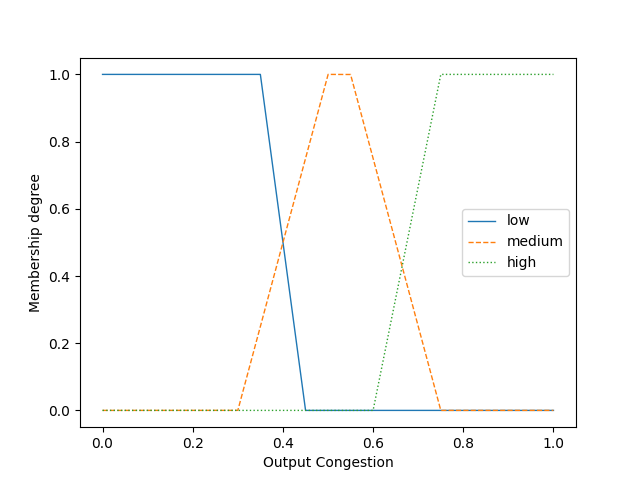
\includegraphics[width=.33\textwidth]{images/plots/OutCongestion.png}\hfill
    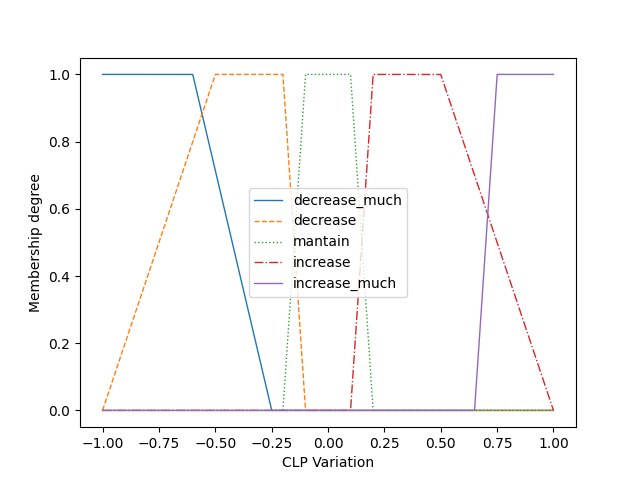
\includegraphics[width=.33\textwidth]{images/plots/CLP.png}

    \hspace*{-1cm}
    \caption{Membership functions for the "CLP Variation" Fuzzy System}
    \label{fig:FS_CLP_FSETS}
\end{figure}


\subsubsection{Fuzzy Rules}
Because the output of our final Fuzzy System is a Fuzzy Set, we decided to use a Mamdani Fuzzy Model, with the fuzzy rules shown in the FAMs \ref{tab:FAM_HDR}, \ref{tab:FAM_OUTC} and \ref{tab:FAM_CLP}.
\begin{itemize}
    \item \textbf{Hardware Resources Fuzzy System}
    \begin{table}[!htb]
        \begin{center}
            \begin{tabular}{ |c|c|c|c|c| }
                \hline
                & & \multicolumn{3}{c|}{Processor Load} \\
                \hline
                \multirow{4}{4em}{Memory}
                &        & Low   & Medium & High\\
                & Low    & L     & M      & H   \\
                & Medium & M     & M      & H   \\
                & High   & H     & H      & VH   \\
                \hline
            \end{tabular}
            \caption{FAM for Hardware Resources Fuzzy Rules}
            \label{tab:FAM_HDR}
        \end{center}
    \end{table}

    \item \textbf{Output Congestion Fuzzy System}
    \begin{table}[!htb]
        \begin{center}
            \begin{tabular}{ |c|c|c|c|c| }
                \hline
                & & \multicolumn{3}{c|}{Output Bandwidth Available} \\
                \hline
                \multirow{4}{4em}{Network Throughput}
                &        & Low   & Medium & High \\
                & Low    & M     & L      & L    \\
                & Medium & H     & M      & M    \\
                & High   & H     & H      & H    \\
                \hline
            \end{tabular}
            \caption{FAM for Output Congestion Fuzzy Rules}
            \label{tab:FAM_OUTC}
        \end{center}
    \end{table}

    \item \textbf{CLP Variation Fuzzy System}
    \begin{table}[!htb]
        \begin{center}
            \begin{tabular}{ |c|c|c|c|c| }
                \hline
                & & \multicolumn{3}{c|}{Output Congestion} \\
                \hline
                \multirow{5}{6em}{Hardware Resources}
                &             & Low   & Medium & High \\
                & Low         & ↑↑    & ↑↑     & ↑↑    \\
                & Medium      & 0     & ↑      & ↓    \\
                & High        & ↓↓    & ↓      & ↓    \\
                & Very High   & ↓↓    & ↓↓     & ↓↓   \\
                \hline
            \end{tabular}
            \caption{FAM for CLP Variation Fuzzy Rules}
            \label{tab:FAM_CLP}
        \end{center}
    \end{table}
\end{itemize}


In figures \ref{fig:FS_CpuMem_OUT}, \ref{fig:FS_OutCongestion_OUT} and \ref{fig:FS_CLP_OUT} are the surfaces induced by the rules for the 3 considered fuzzy systems.

\begin{figure}[!htb]
    \centering

    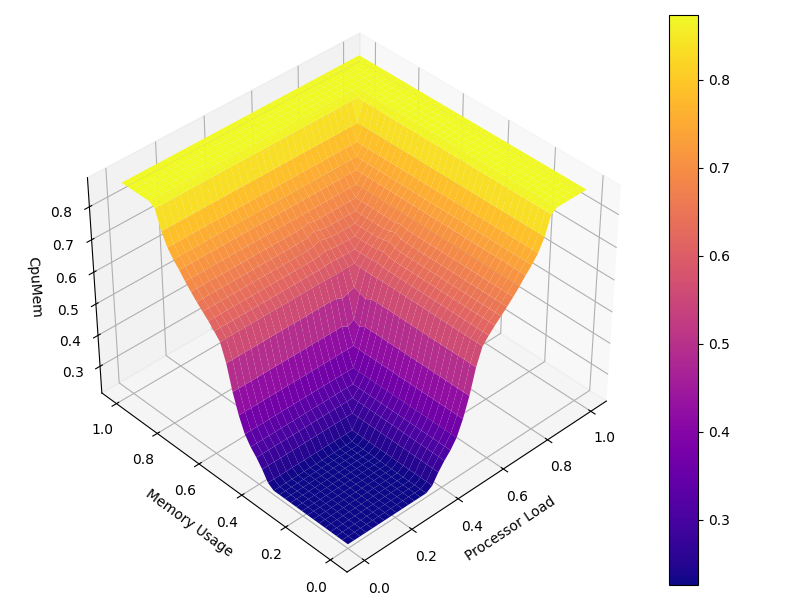
\includegraphics[width=.6\textwidth]{images/plots/CpuMem3D_better.png}\hfill

    \caption{Surface induced by the Hardware Resources Fuzzy System}
    \label{fig:FS_CpuMem_OUT}
\end{figure}

\begin{figure}[!htb]
    \centering

    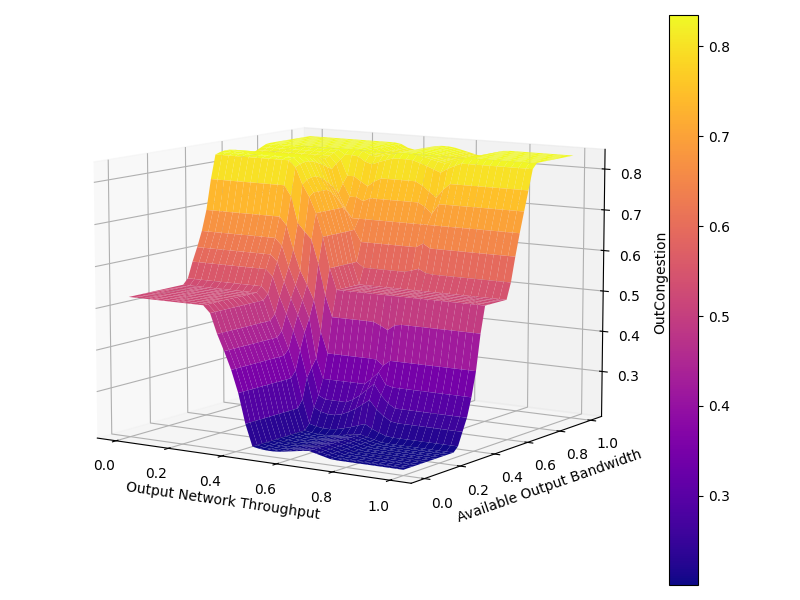
\includegraphics[width=.6\textwidth]{images/plots/OutCongestion3D.png}\hfill

    \caption{Surface induced by the  Output Congestion Fuzzy System}
    \label{fig:FS_OutCongestion_OUT}
\end{figure}

\begin{figure}[!htb]
    \centering

    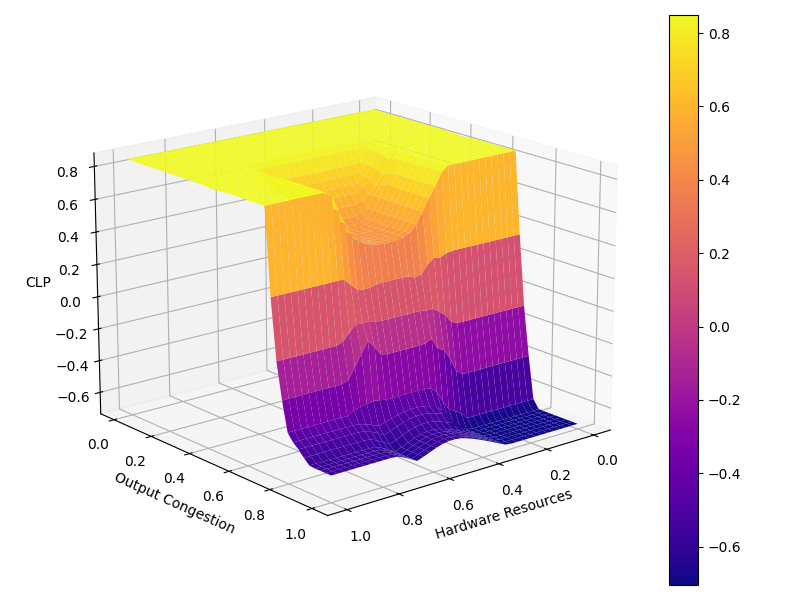
\includegraphics[width=.6\textwidth]{images/plots/CLP3D_better.png}\hfill

    \caption{Surface induced by the Computing Load Variation Fuzzy System}
    \label{fig:FS_CLP_OUT}
\end{figure}

\newpage

\subsection{Testing and Results}

In refining our fuzzy system, we implemented several strategic adjustments to enhance its performance. Firstly, we meticulously modified the rule set to match better our anticipated output, ensuring a more precise correspondence between input variables and system responses. Additionally, we meticulously fine-tuned the trapezoid points, strategically adjusting them to optimize the system's accuracy and efficacy in generating outputs. As a direct outcome of these refinements, we observed a notable improvement in the system's overall performance. However, it's worth noting a particular consequence of these enhancements: our parameter "decrease much" has now a minimum of at -0.6. Even though the rules are effectively being applied as intended, this intrinsic limitation implies that our system's \textit{CLP Variation} cannot extend beyond this threshold.

For the dataset provided, we obtained the results in table \ref{tab:RESULTS_CLP}.
\begin{table}[H]
    \begin{center}
        \begin{tabular}{ |c|c| }
            \hline
            Predicted & Expected \\
            \hline
            84\% & 85\% \\
            85\% & 85\% \\
            85\% & 80\% \\
            81\% & 73\% \\
            59\% & 50\% \\
            52\% & 12\% \\
            -49\% & -31\% \\
            -49\% & -65\% \\
            -53\% & -82\% \\
            -57\% & -85\% \\
            \hline
        \end{tabular}
        \caption{Predicted vs Expected \textit{CLP Variation}}
        \label{tab:RESULTS_CLP}
    \end{center}
\end{table}

As we can see in Table \ref{tab:RESULTS_CLP}, the last 2 lines of the table have a big discrepancy because our system cannot output values below -0.6. The only line that requires more attention is the \nth{6}, where our output is 52\% and the expected value is 12\%. After analyzing the data, we concluded that with the variables we chose to use for our system, we are unable to provide a different output. Only a system with more inputs could produce a closer output to the expected values.


\newpage

\section{Neural Networks}
% Present the NN model and the rationale you used to build, train, validate and test it (including the generation of the dataset).

\subsection{Introduction}

The objective is to implement a model based on a Multilayer Neural Network (NN) to control the variation of the Computing Load Percentage (CLPVariation), given some system parameters as input (such as memory, processor, network, etc...).
This neural network should model the Fuzzy System developed in section \ref{sec:fuzzy_system}.


\subsection{Datasets}
The datasets used to build the model were generated using a randomized script and the Fuzzy System previously mentioned.

First, we developed a script to randomize the inputs of the fuzzy system, and then feed them to the fuzzy system to obtain the expected output of the neural network.

To avoid overfitting the model, we must use 3 datasets: Training, Validation and Test.
Instead of generate a mega-dataset and split it, because we wanted to cover the input space uniformly, we decided to generate the datasets independently, knowing that that the points shouldn't overlap in the datasets (that is, there shouldn't be the same inputs in the 3 datasets).

With "cover the input space uniformly" in mind, we decided to generate the points sequentially for the training dataset, to avoid clusters and obtain a balanced dataset. First, we generated numbers using 11 training points for each of the 4 used features \textit{(Processor Load, Memory Usage, Output Throughput and Output Bandwidth)}, generating numbers with a 0.1 interval (between 0 and 1), and randomized the values for the variations and the unused features, as these values wouldn't be used anyway as an input of the model. This created a dataset with $11^{4} = 14 641$ examples.

To validate and test the model, we decided to use truly random values for all the features, so we generated a data set with 10 000 000 points, and split it 50/50, to originate our Validation and Test Datasets.


\subsection{Regression problem}

The neural network is expected to replicate the results of the Fuzzy System. This is a regression problem, as the goal is to predict a quantitative value.


\subsubsection{NN model}

To begin training the model, we used a MLPRegressor model, with the \textit{logistic} activation function and the \textit{sgd} (stochastic gradient descent) solver.
Next, it was needed to tune the parameters and hyperparameters of the model (number of inputs, number of hidden layers, etc), so we developed a script to iterate over them and find the best values.
We started by testing our model by hand for a single hidden layer of 1 to 8 neurons and concluded that 5 neurons gave the lowest \textit{mean squared error} as we can see in Table \ref{tab:MSE_5_log_sgd}.

\begin{table}[H]
    \centering
    \begin{tabular}{l|l|}
        \cline{2-2}
                                       & MSE       \\ \hline
        \multicolumn{1}{|l|}{Validate} & 0.0697423 \\ \hline
        \multicolumn{1}{|l|}{Test}     & 0.07008434  \\ \hline
    \end{tabular}
    \caption{Mean Square Error for 5 neurons with logistic activation and sgd solver}
    \label{tab:MSE_5_log_sgd}
\end{table}

We then used \textit{Grid Search} to optimize the parameters and discovered that this approach yielded improved results. Specifically, we achieved better performance with \textit{activation='relu' and solver='adam'} compared to the original settings of \textit{activation='logistic' and solver='sgd'}.

After that, we tested for combinations of 1 and 2 hidden layers and tested from 1->20 neurons on a single or 2 layers, and we reached the lowest error at 8 neurons on the first layer and 3 neurons on the second.

\begin{verbatim}
    INFO: Best parameters found: {'activation': 'relu', 'alpha': 0.0001,
    'hidden_layer_sizes': (8, 3), 'learning_rate': 'constant', 'max_iter': 2000,
    'solver': 'adam'}
    INFO: Mean Squared Error with best parameters: 0.016218705321498234
\end{verbatim}

From the output of the Grid Search function above, we obtain the final results: 2 hidden layers, the first with 8 nodes, the second with 3, \textit{relu} activation function and the \textit{adam} solver.

We trained our final model (illustrated in Figure \ref{fig:NN_diagram}) using these parameters and the training dataset. With this model, the Mean Squared Error for the validation dataset is 0.0162187.

\begin{figure}[H]
    \centering
    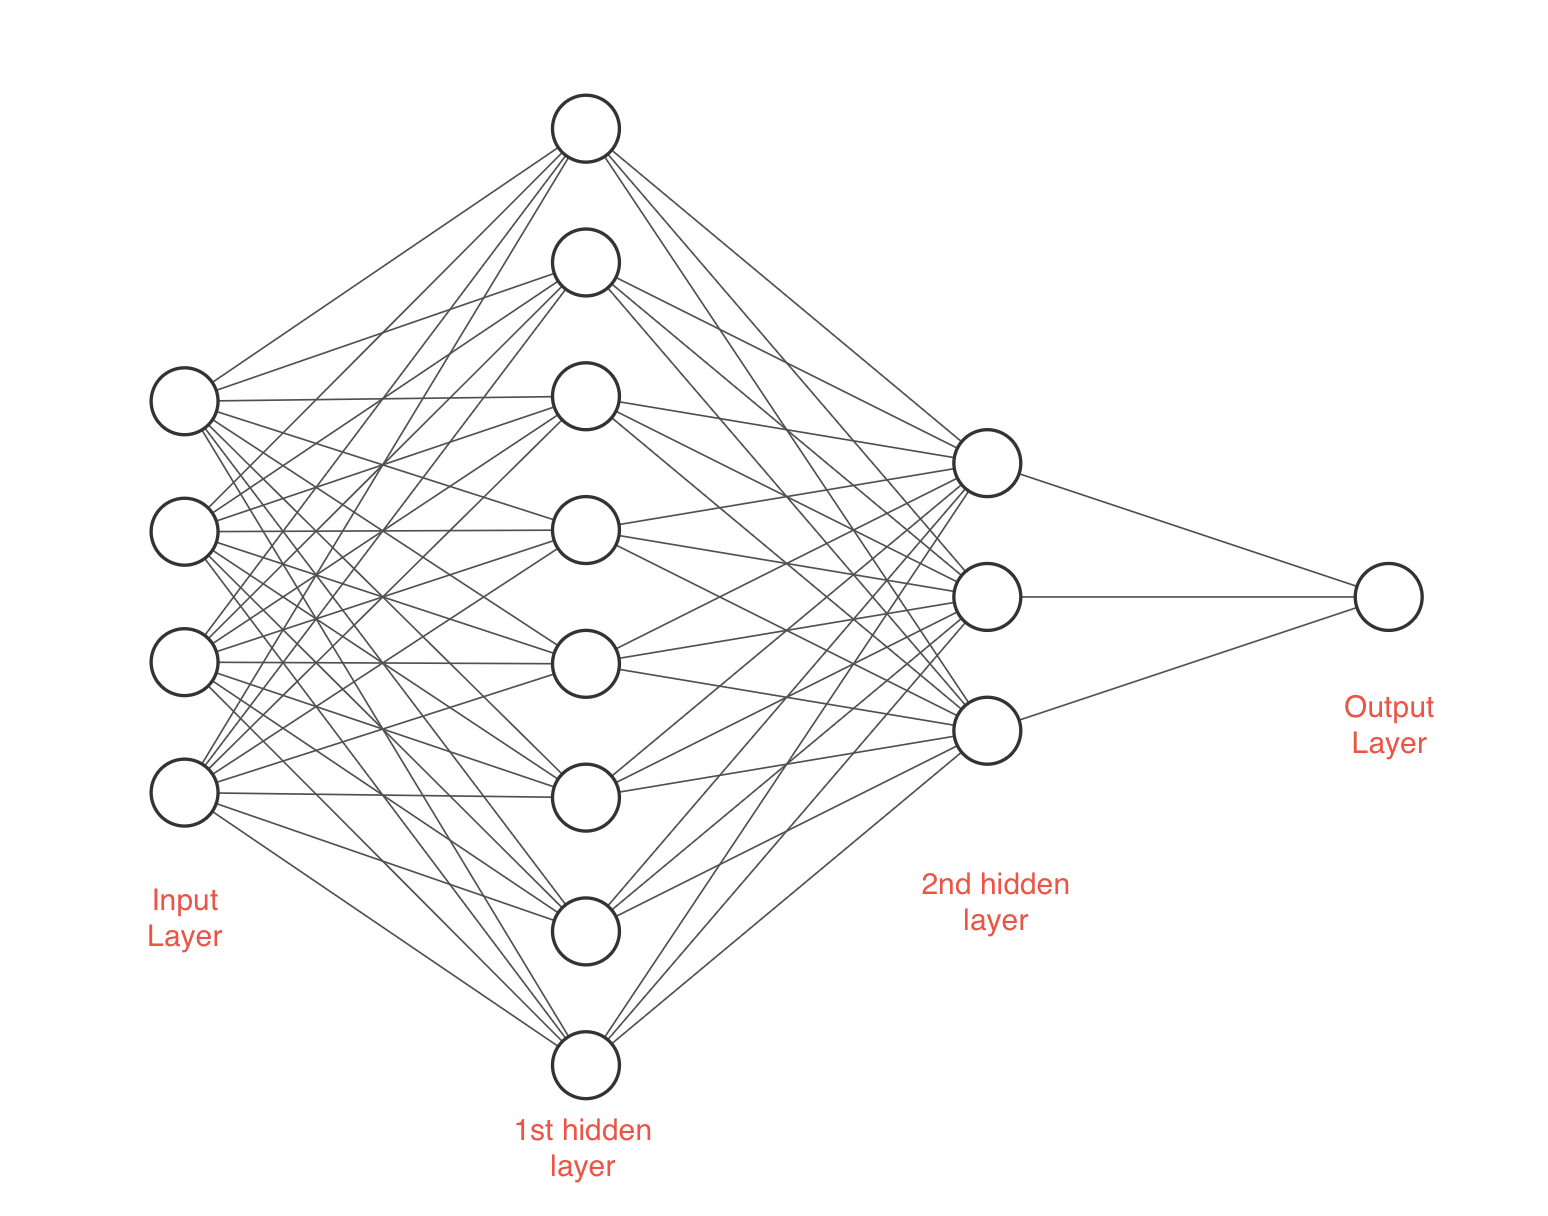
\includegraphics[width=\textwidth]{images/NN_diagram.png}
    \caption{Visual representation of the final Neural Network}
    \label{fig:NN_diagram}
\end{figure}


\subsection{Results}

To evaluate our final model, we tested it against our Test dataset. The results are presented in Table \ref{tab:MSE_11_relu_adam}.

\begin{table}[H]
    \centering
    \begin{tabular}{l|l|}
        \cline{2-2}
                                       & MSE       \\ \hline
        \multicolumn{1}{|l|}{Validate} & 0.0162187 \\ \hline
        \multicolumn{1}{|l|}{Test}     & 0.0162200 \\ \hline
    \end{tabular}
    \caption{Mean Square Error for 8+3 neurons with relu activation and adam solver}
    \label{tab:MSE_11_relu_adam}
\end{table}

The mean squared error (MSE) of the model on the test set is calculated to be 0.0162200. This metric provides insight into the average squared difference between the actual and predicted values. A lower MSE indicates better model performance, with values closer to zero indicating a more accurate prediction. In this case, the MSE suggests that the model's predictions deviate from the actual values by an average squared error of approximately 0.016. We can also see that the 2 values for the errors are very similar, which suggests for once that the two datasets are similarly balanced, and twice that the final model should be a good model (without overfitting), predicting correctly any new value, that it hasn't been "seen" yet.

\begin{figure}[H]
    \centering
    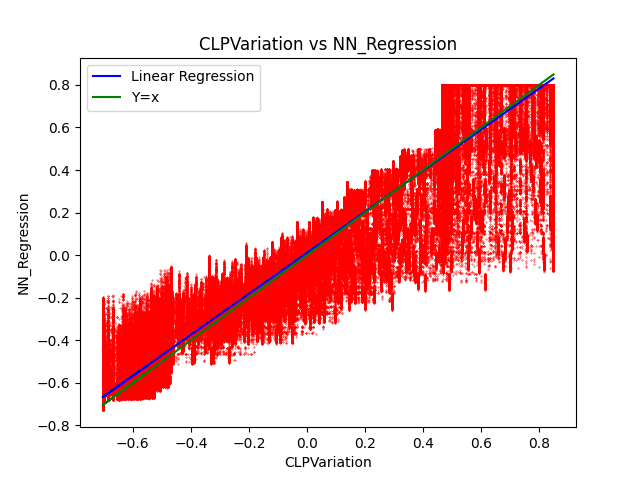
\includegraphics[width=\textwidth]{images/CLP vs Regression.png}\hfill
    \caption{Linear Regression Expected CLP vs Neural Network Prediction}
    \label{fig:FS_NN_LIN_REG}
\end{figure}

Figure \ref{fig:FS_NN_LIN_REG} shows the representation of the linear regression of our model, the green line the regression of a perfect model. We expected the red points to fall near the green line. We can see that that is the case for the most points, given for the compact red areas around the line.
However, we can also see that there are some outliers present, where some red dots deviate from the line on the right of the graph: where the model should predict a very high CLPVariation (> 0.5), is predicting a moderate increase (between 0 and 0.4). Although this might be a concerning issue, because the MSE that we got is so low, we shouldn't be concerned.
In practical terms, this just means that we aren't using the Edge device capabilities to their possible maximum and also aren't contradicting the expected data. This suggests that the edge device should still be able to achieve its purpose effectively. While there may be slight deviations in the predictions, they remain within acceptable bounds, ensuring the continued functionality and reliability of the system.

\newpage

\subsection{Classification problem}
% Increase, decrease or maintain (classes)

We now want to use the NN as a multiclass classifier with the following 3 classes: “Decrease”, “Maintain”, “Increase”.

To achieve that, we created a function (classification function) that maps the CLPVarition values to the 3 classes. The limits for this function are expressed in Table \ref{tab:classifications}.

\begin{table}[H]
    \centering
    \begin{tabular}{|l|l|l|}
        \hline
        Class    & Lower Bound & Upper Bound  \\
        \hline
        Decrease & $-\infty$   & $-0.2$       \\
        \hline
        Maintain & $-0.2$      & $0.2$        \\
        \hline
        Increase & $0.2$       & $\infty$     \\
        \hline
    \end{tabular}
    \caption{Classification Bounds}
    \label{tab:classifications}
\end{table}

For this problem, we ran the NN model against the 3 datasets (Training, Validation and Test), and feed the output from the model to our classification function. To evaluate the results, we also feed the "correct" values to the classification function, and computed the classification metrics.

\subsubsection{Results}

% Key Metrics Explained:
% Precision: The ratio of correctly predicted positive observations to the total predicted positives. High precision indicates a low false positive rate.
% Recall: The ratio of correctly predicted positive observations to the all observations in the actual class. High recall indicates a low false negative rate.
% F1-Score: The weighted average of Precision and Recall. The F1 Score is especially useful when the class distribution is imbalanced.
% Support: The number of actual occurrences of the class in the dataset.

In tables \ref{tab:classification_report_train} through \ref{tab:confusion_matrix_test} are the classification reports (precision, recall, F1-score and accuracy metrics) and the confusion matrices for the 3 datasets, providing a detailed insight into the performance of the neural network model across the three defined classes: 'Decrease', 'Maintain', and 'Increase'.

%%%%%%%%%%%%%%%%TRAIN%%%%%%%%%%%%%%%%%%

\begin{table}[H]
\centering
\begin{tabular}{|l|l:l:l:l|}
\cline{2-5}
\multicolumn{1}{l|}{} & \multicolumn{1}{l|}{Precision} & \multicolumn{1}{l|}{Recall} & \multicolumn{1}{l|}{F1-score} & support               \\
\hline
Decrease              & 0.92                           & 0.95                        & 0.94                          & 5989               \\
\cline{1-1}
Increase              & 1.00                           & 1.00                        & 1.00                          & 7744                \\
\cline{1-1}
Maintain              & 0.60                           & 0.47                        & 0.53                          & 908               \\
\hline
\multicolumn{1}{l}{}  &                                &                             &                               & \multicolumn{1}{l}{}  \\
\hline
accuracy              &                                &                             & 0.95                          & 14641               \\
\cline{1-1}
macro avg             & 0.84                           & 0.81                        & 0.82                          & 14641               \\
\cline{1-1}
weighted avg          & 0.94                           & 0.95                        & 0.95                          & 14641               \\
\hline
\end{tabular}
    \caption{Classification Report for Training dataset}
    \label{tab:classification_report_train}
\end{table}

\begin{table}[H]
\centering
\begin{tabular}{|cc|c:c:c|} 
\cline{3-5}
\multicolumn{1}{c}{}               &          & \multicolumn{3}{c|}{Predicted}                                          \\
\multicolumn{1}{c}{}               &          & \multicolumn{1}{c}{Decrease} & \multicolumn{1}{c}{Increase} & Maintain  \\ 
\hline
\multirow{3}{*}{Actual} & Decrease & 5703                         & 0                            & 286       \\ 
\cdashline{3-5}
                                   & Increase & 0                            & 7744                         & 0         \\ 
\cdashline{3-5}
                                   & Maintain & 478                          & 0                            & 430       \\
\hline
\end{tabular}
\caption{Confusion Matrix for Training dataset}
    \label{tab:confusion_matrix_train}
\end{table}

The classification report for the training set, summarized in table \ref{tab:classification_report_train}, demonstrates exceptional performance in predicting the 'Decrease' and 'Increase' classes, with precision and recall values both around 0.92 and 1.00 respectively. This indicates that the model is highly accurate in identifying instances where the output is either 'very negative' or 'very positive', with zero false-positives and false-negatives in the 'Increase' class.
This is expected, as this is the dataset used for training the Neural Network, where the weighs are computed to be the very best to meet the excepted output.

%%%%%%%%%%%%%%%%VALIDATE%%%%%%%%%%%%%%%
\begin{table}[H]
\centering
\begin{tabular}{|l|l:l:l:l|}
\cline{2-5}
\multicolumn{1}{l|}{} & \multicolumn{1}{l|}{Precision} & \multicolumn{1}{l|}{Recall} & \multicolumn{1}{l|}{F1-score} & support               \\
\hline
Decrease              & 0.98                           & 0.97                        & 0.97                          & 1859972               \\
\cline{1-1}
Increase              & 0.98                           & 0.98                        & 0.98                          & 2825928                \\
\cline{1-1}
Maintain              & 0.68                           & 0.74                        & 0.71                          & 314100               \\
\hline
\multicolumn{1}{l}{}  &                                &                             &                               & \multicolumn{1}{l}{}  \\
\hline
accuracy              &                                &                             & 0.96                          & 5000000               \\
\cline{1-1}
macro avg             & 0.88                           & 0.90                        & 0.89                          & 5000000               \\
\cline{1-1}
weighted avg          & 0.96                           & 0.96                        & 0.96                          & 5000000               \\
\hline
\end{tabular}
    \caption{Classification Report for Validation dataset}
    \label{tab:classification_report_validate}
\end{table}

\begin{table}[H]
\centering
\begin{tabular}{|cc|c:c:c|} 
\cline{3-5}
\multicolumn{1}{c}{}               &          & \multicolumn{3}{c|}{Predicted}                                          \\
\multicolumn{1}{c}{}               &          & \multicolumn{1}{c}{Decrease} & \multicolumn{1}{c}{Increase} & Maintain  \\ 
\hline
\multirow{3}{*}{Actual} & Decrease & 1794895                        & 0                               & 65077       \\ 
\cdashline{3-5}
                                   & Increase & 211                            & 2782793                         & 42924         \\ 
\cdashline{3-5}
                                   & Maintain & 33844                          & 47120                           & 233136       \\
\hline
\end{tabular}
\caption{Confusion Matrix for Validation dataset}
    \label{tab:confusion_matrix_validate}
\end{table}

%%%%%%%%%%%%%%%%TEST%%%%%%%%%%%%%%%%%%%
\begin{table}[H]
\centering
\begin{tabular}{|l|l:l:l:l|}
\cline{2-5}
\multicolumn{1}{l|}{} & \multicolumn{1}{l|}{Precision} & \multicolumn{1}{l|}{Recall} & \multicolumn{1}{l|}{F1-score} & support               \\
\hline
Decrease              & 0.98                           & 0.96                        & 0.97                          & 1858190               \\
\cline{1-1}
Increase              & 0.98                           & 0.98                        & 0.98                          & 2827993                \\
\cline{1-1}
Maintain              & 0.68                           & 0.74                        & 0.71                          & 313817               \\
\hline
\multicolumn{1}{l}{}  &                                &                             &                               & \multicolumn{1}{l}{}  \\
\hline
accuracy              &                                &                             & 0.96                          & 5000000               \\
\cline{1-1}
macro avg             & 0.88                           & 0.90                        & 0.89                          & 5000000               \\
\cline{1-1}
weighted avg          & 0.96                           & 0.96                        & 0.96                          & 5000000               \\
\hline
\end{tabular}
    \caption{Classification Report for Test dataset}
    \label{tab:classification_report_test}
\end{table}

\begin{table}[H]
\centering
\begin{tabular}{|cc|c:c:c|} 
\cline{3-5}
\multicolumn{1}{c}{}               &          & \multicolumn{3}{c|}{Predicted}                                          \\
\multicolumn{1}{c}{}               &          & \multicolumn{1}{c}{Decrease} & \multicolumn{1}{c}{Increase} & Maintain  \\ 
\hline
\multirow{3}{*}{Actual} & Decrease & 1792873                        & 0                               & 65317       \\ 
\cdashline{3-5}
                                   & Increase & 250                            & 2784752                         & 42991         \\ 
\cdashline{3-5}
                                   & Maintain & 33923                          & 47101                           & 232793       \\
\hline
\end{tabular}
    \caption{Confusion Matrix for Test dataset}
    \label{tab:confusion_matrix_test}
\end{table}

Because the Validation and Test datasets share the same results, they are analysed together.
Both for the Validation and Test dataset, it is observed a high precision, recall and F1-score for the "Decrease" and "Increase" classes, with values between 0.96 and 0.98. However, the model's performance for the 'Maintain' class is notably lower, with a precision of 0.68 and recall of 0.74, resulting in an F1-score of 0.71 (for the 2 datasets). This suggests that the model has difficulty distinguishing instances where the output is closer to 0, leading to a higher rate of misclassification in this category. This discrepancy is likely due to the class imbalance in the dataset, where the 'Maintain' class has significantly fewer samples compared to the 'Decrease' and 'Increase' classes.

The overall accuracy of the model stands at 96\%, which indicates that the majority of the predictions are correct. The macro average metrics, which treat all classes equally, show slightly lower values (precision: 0.88, recall: 0.90, F1-score: 0.89), reflecting the model's challenges with the 'Maintain' class. In contrast, the weighted average metrics, which consider the number of instances per class, align closely with the high overall accuracy, as the performance on the dominant classes ('Decrease' and 'Increase') heavily influences these averages.

Additionally, the confusion matrix for the Test dataset, as shown in table \ref{tab:confusion_matrix_test}, further illustrates the model's performance by summarizing the number of correct and incorrect predictions for each class. The confusion matrix reveals that the model accurately predicts the 'Decrease' and 'Increase' classes, with a large number of true positive predictions (1,792,873 and 2,784,752, respectively) and relatively low false positive and false negative predictions. However, the model struggles more with the 'Maintain' class, as evidenced by the higher number of false positive and false negative predictions compared to the other classes. These insights from the confusion matrix help identify areas for improvement and guide future refinements to enhance the model's predictive capabilities.


\end{document}
